\chapter{Introduction} \label{ch:intro}
% Word checked, no spell and gramma error. 
For any autonomous vehicle, generating an accurate and high precision
model of its surrounding environment to indicate hazard features, and
knowing its own location in the map is essential for the vehicle to
navigate and avoid obstacles autonomously.

In many applications, the mobile robot has an a priori map. The given
a priori map may be sufficient for localization purposes, but generally
does not have sufficient resolution or up-to-date information for
obstacle detection. Ground vehicles need to deal with temporary added
road blocks and parked cars. Aerial vehicles need a high resolution map
that indicates tall trees, steep hills or electrical towers. In
addition, a usable map does not always exist. Without maps and
externally referenced pose information, the robot must produce its own
map and concurrently localize itself within the map. This problem is
referred to as simultaneous localization and mapping (SLAM).

Traditional two-dimensional SLAM algorithms have been well established in
the past decade. A SLAM algorithm typically utilises measurements from
several types of sensors which can be divided into two groups: those
that provide vehicle pose measurements, such as a wheel odometer or
GPS; and those that provide landmark bearing and range measurements,
such as radar, sonar, laser range finder. In recent years, optical
sensors are actively being incorporated into SLAM algorithms and
successfully used in ground vehicle navigation. For aerial vehicles,
the experiments are mostly limited to
simulation\cite{nemra_robust_2010} \cite{jianli_unscented_2011}
\cite{sunderhauf_using_2007} \cite{artieda_visual_2009}, and results
from realistic aerial video data are rare.

\section{Problem Statement}\label{section:ProblemStatement}
% Word checked.
Obstacle detection (OD) has received a lot of research interest in
recent years. Various algorithms were developed for ground, under
water and aerial vehicles using different sensors such as sonar, radar,
LIDAR, and vision. Most OD system focused on only one sensor. Yet,
using multiple sensors generally produced better measurements than
a single sensor \cite{smith_approaches_2006}. On most unmanned aerial
vehicle (UAV) platforms, many sensors are readily available, such as
accelerometers, gyroscope, GPS receiver, altimeter, etc. Fully
utilizing these sensors should improve the accuracy and robustness of
an OD system, especially in harsh flying conditions.

This thesis focused on developing and testing an obstacle detection system by
using a SLAM algorithm as a sensor fusion framework to integrate
measurements from various sensors on a typical UAV navigation device.
The type of application targeted by this work is a medium size UAV
conducting low altitude terrain following flight in a natural
environment. The obstacles are static objects on ground; moving
objects are not considered. Research presented in this thesis
contributed to the project of developing a mid-size UAV to perform
geological surveys, carried out by Carleton University in
collaboration with Sander Geophysics Ltd. which is an Ottawa based
company specializing in high precision geophysical survey. To achieve
high resolution data acquisition, the UAV must be able to perform
terrain following flight with altitude as low as 10 meters from
ground, and with a ground speed ranging from 60 knots (30.87 m/s) to 100
knots (51.44 m/s). The specified rate of climb for the UAV is 400ft of
vertical rise per minute (122 meters per minute)
\cite{james_geosurv_2008}. A quick analysis on the UAV specification
and aerodynamic behavior reveals the detection requirement of the OD
system. Assuming a tree height of 20 meters, which is the average
height for oak or pine, to allow for enough time to avoid obstacle,
the UAV must be able to detect the threat at 610 meters or further
(Figure \ref{ob}). This analysis indicates that the obstacle detection
must be able to map objects up to a thousand meters from the UAV.

\begin{figure}[h]
\centering
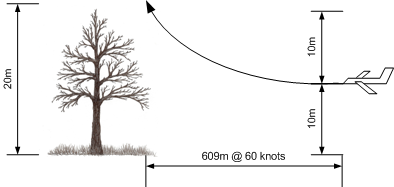
\includegraphics[width=300pt,height=160pt]{./Figures/ProblemStatement.png}
\caption {Case study for obstacle detection requirement}
\label{ob}
\end{figure}

Although digital terrain maps are generally available for flight path
planning and in-flight navigation, they do not have the resolution to
indicate all hazardous obstacles such as tall trees, steep hills, or
man-made objects. The obstacle detection and avoidance system must be
in place to detect discrete threats, and to operate automatically with
minimum intervention from the operator.

\section{Contributions}\label{section:Contribution}
% word checked.
The thesis first reviews the pros and cons of various sensors, and
points out the advantages and disadvantages of using imaging sensors in
an OD application. Different types of imaging sensor configurations and
sensor calibration methods are also described. Next, the thesis
reviews the formulation and properties of a typical extended Kalman
filter (EKF) based SLAM algorithm, and discusses the advantages and
limitations of an EKF based SLAM algorithm.

The reviews and discussions lead to implementation of an improved EKF
SLAM method by fusing multiple sensors with monocular camera video.
%Using a monocular vision for mapping is a bearing only
%problem. The measurement is through projection, which loses
%information about the relative position of the feature since the range
%is unknown. Without camera motion measurements, map created by
%monocular vision can be scaled arbitrarily. 
A camera centric EKF based SLAM algorithm (referred to as CC-EKF-SLAM
in the rest of the article) is described in this thesis. The
algorithm utilizes an extended Kalman filter to fuse camera motion
measurements from inertial and gyroscope sensors and landmark
measurements from video of a single wide angle camera. Inverse
parameterization was adopted to describe the landmark positions so
that distant landmarks can be estimated. Camera centric coordinate system
were used to improve the consistency of the framework for large area
mapping. The filter can estimate absolute coordinates of landmarks and
the poses of the UAV directly. An interpolated map can be generated
from the estimates to represent the surrounding environment of the
UAV, and the location of the UAV within it.

To test the algorithm under true flying condition, aerial flight data
were collected and processed by the CC-EKF-SLAM algorithm. To capture
low altitude flight video and navigation data, a simulated unmanned
aerial system (SUAS) with various sensors on-board was towed by a
helicopter which flew a pre-planned path in the mountain north of
Gatineau, Quebec. Sensors installed included 1 CCD camera with 6mm
focal length lens, GPS antenna, a UAV navigation module with embedded
accelerometer, gyroscope, GPS receiver, and external fluxgate sensor.
The helicopter flew at a speed of 60 knots, and at an altitude of 100
meters above ground, with the SUAS at approximately 70 meters above
ground. Two pieces of video and data were processed by the CC-EKF-SLAM
algorithm. The result proved that the CC-EKF-SLAM algorithm was
capable of mapping landmarks over 1000 meters away. The preliminary
result of the test flight was published in \cite{zhang_obstacle_2012}.
This paper was one of the first in the field that successfully applied
monocular vision SLAM in large scale aerial OD application.

To further analyze errors seen in the flight test results, a series
of simulations were done to thoroughly study the behavior of the
algorithm under various circumstances, including
\begin{itemize}
\item UAV conducting simple forward motion
\item UAV experiencing oscillatory motion on all other 5 degree of
freedom (DOF)
\item error in camera calibration
\item quantization error introduced through image digitization 
\end{itemize}
The results of these simulations are valuable to the design of data
acquisition hardware for obstacle detection purposes, and to the future
improvement of the CC-EKF-SLAM algorithm.

\section{Organization}\label{section:Organization}
% word checked
The thesis is organized as follows:

\begin{itemize}
  \item Chapter 2 presents an overview on sensors, and data fusion
  framework (EKF and SLAM) related to obstacle detection and range
  measurement.
  \item Chapter 3 describes the experiment setup for the aerial data
  collection, camera calibration procedure and result, and ground
  truth data collection.
  \item Chapter 4 describes the detailed implementation of the proposed
  CC-EKF-SLAM algorithm. Data preparation steps used to compare
  estimated data with the ground truth are also given in this chapter.
  \item Chapter 5 presents the results of the flight test. Convergence and
  consistency of the algorithm are discussed. Accuracy analysis by
  comparing to the ground truth data is also presented.
  \item Chapter 6 presents the results of error analysis through
  simulations. Behavior of the CC-EKF-SLAM
  algorithm was studied through simulating a number of scenarios.
  \item Chapter 7 gives an overall summary of the results obtained in
  this research, and recommendations for future research.
\end{itemize}

%%% Local Variables:
%%% mode: latex
%%% TeX-master: "thesis.tex"
%%% End:
